\documentclass{article}
% document class two side means margins are set for book like documents
% report means you can use Chapters book also the same
% article can only use sections.

%package list and settings!

\usepackage{float} 
%required for the figures and tables to be located as intended 
% USE [!ht] after tables or figures => \begin{figure}[!ht]

\usepackage{ulem}
% required for strikethrough or any line stikes wavy lines accessories 

\usepackage{amsmath}
% additional for math formulas typing

\usepackage{caption}
\usepackage{subcaption}
% required for making captions (auto numbering) for figures and tables
% the numbering is depends on the documentclass input  
% if this is report the caption is use the Chapter and sequence in the chapter
% for article is the section used for numbering.

\usepackage{graphicx}
% this package is used to \includegraphics[width=...\textwidth]{path}
\graphicspath{{./images/}}

\usepackage{geometry}
% this package supposedly to give the user ability to change margins-spaces settings.

\usepackage{hyperref}
% hyperlink packages used mostly for \href{URL}{text}
\hypersetup{colorlinks=true, linkcolor=blue}

\usepackage{color}
\definecolor{anti-flashwhite}{rgb}{0.95, 0.95, 0.96}


\usepackage{listings}
% this package is to facilitate code highlighting for certain programming language
% WARNING: NOT ALL PROGRAMMING LANGUAGES ARE SUPPORTED BY THIS LINTER.
% NOTE: You can customize the linter yourself using:
% \lstdefinestyle{name of style}{key value data on properties.}
\lstset{ % General setup for the package
    language=Python,
    basicstyle=\small\ttfamily,
	backgroundcolor=\color{anti-flashwhite}
    numbers=left,
     numberstyle=\tiny,
    frame=tb,
    tabsize=4,
    columns=fullflexible,
    breaklines=true,
    postbreak=\mbox{\textcolor{red}{$\hookrightarrow$}\space},
    showstringspaces=false,
    showtabs=false,
    keepspaces,
    commentstyle=\color{red},
    keywordstyle=\color{blue}
}


\title{Lecture 2 Project: Document Distance}
\author{Yanuar Heru Prakosa}
\date{31-05-2021}

\begin{document}
    \maketitle

    \section*{The Document Distance}
    The assignment from the Lecture 2 in 6-006 is related to one called document distance. 
    Thus I need to find out first what is exactly document distance is.  
    \href{http://6.006.scripts.mit.edu/~6.006/spring08/wiki/index.php?title=Document_Distance_Problem_Definition}{Form this MIT discussion webpage}, I learn that document distance will be measured using vector equations.
    Let D be a text, then a word is a consecutive of alphanumeric characters. 
    We will not distinguish upper case and lower case letters, but we use non alphanumeric characters as delimiter between words.
    For example the word "can't" consist of 2 words: can and t.
    
    Okay now we go to the formulation:
    The word \emph{word frequency distribution} of a document D ia a mapping from words \emph{w} to their frequency count, denoted as $D(w)$.
    We can view the frequency distribution D as vector, with one component per possible word. Each component will be a non-negative integer $\geq 0$.

    The norm of this vector is defined by:
    \begin{equation*}
        N(D) = \sqrt{D \cdot D} = \sqrt{\sum_{w}{D(w)^{2}}}
    \end{equation*}
    Alright this calculation still does not make any sense right now.
    But let's move on, I need to get to how to calculate document distance first.
    Now when we have two documents to be compared to each other, let's name them $D$ and $D'$. 
    The inner product between $D$ and $D'$ is defined as:
    \begin{equation*}
        D \cdot D' = \sum_{w}{D(w)D'(w)}
    \end{equation*}
    So basically this is the sum of products on all word frequencies in two documents.
    Thus, if a word exist 1000 times in one document but never existed in other document the inner product of that part is 0!

    Okay, since our objective is to define distance which is defined here as angle between two documents we need to go back to definition of vector dot products:
    \begin{equation*}
        D \cdot D' = N(D) N(D') cos \theta
    \end{equation*}
    As we looking for an angle we are focusing on $\theta$ right?
    Therefore:
    \begin{equation*}
        cos \theta = \frac{D \cdot D'}{N(D)N(D')}
    \end{equation*}
    \begin{equation*}
        \theta = arccos \left( \frac{D \cdot D'}{N(D)N(D')} \right)
    \end{equation*}
    Deriving from other equations above we will get:
    \[
      \theta = arccos \left( \frac{\sum_{w}{D(w)D'(w)}}{\sqrt{\sum_{w}{D(w)^{2}}} \sqrt{\sum_{w}{D'(w)^{2}}}}\right)  
    \]
    From those formula we can infer that if both Documents are the same then the $angle(D,D') = \theta = 0$.
    On the other hand if both documents are completely different in the sense there are no similarity in terms of word used in it then the $angle(D,D') = \theta = \frac{\pi}{2}$. Please note we are using \emph{radians} in this matter.

    \section*{Pre Example}
    To make it clearer I think a simple practical example is mandatory. 
    Let us have two sentences that we will use as documents. 
    One is "To be or not to be" and the other is "Doubt truth to be a liar". 
    We will calculate the distance between these two documents.

    Now we already list all unique set of words and it can be seen in this table plus its frequencies: 
    \textit{FYI: this table is the Document vectors for Document 1 and Document 2}
    \begin{center}
        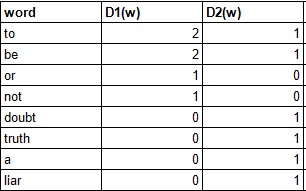
\includegraphics{table word frequencies}    
    \end{center}
        
    Now let's get back to the formula: 
    \[
      \theta = arccos \left( \frac{\sum_{w}{D(w)D'(w)}}{\sqrt{\sum_{w}{D(w)^{2}}} \sqrt{\sum_{w}{D'(w)^{2}}}}\right)  
    \]
    we begin with the denominator part first.

    \newpage
    To calculate the denominator we need to find $\sum_{w}{D(w)^{2}}$ and $\sum_{w}{D'(w)^{2}}$ first. Here is the results of the calculation:
    \begin{center}
        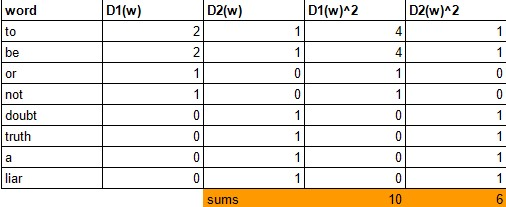
\includegraphics{square frequencies table.jpg}
    \end{center}

    As you can see the sums already being included in the table above.
    We can use it as our denominators, but remember those sum products must be subject to a square root operations.
    Now we need to calculate the nominator side: $sum{D(w)D'(W)}$, which we have already calculated also using spreadsheet:
    \begin{center}
        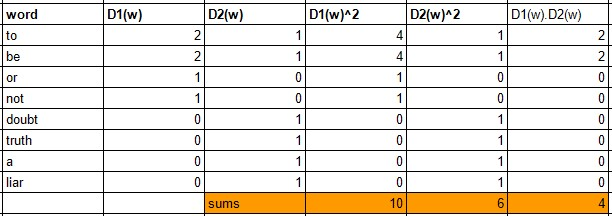
\includegraphics[scale=0.8]{inner product sum table.jpg}
    \end{center}

    As you can see on the table above the $sum{D(w)D'(W)} = 4$, now we can put all of them in the formula:
    \[\theta = arccos \left( \frac{4}{\sqrt{10} \sqrt{6}}\right)\]
    \[\theta = arccos \left( \frac{4}{\sqrt{10.6}}\right)\]
    \[\theta = arccos\left( 0.52\right)\]
    \[\theta = 1.028157225\]

    There you are, that is in summary how we will measure the distance between to documents. 

    \section*{Summary}
    Here is what you should do when measuring the distance between two documents:
    \begin{enumerate}
        \item list all words in a set, meaning there are no double words in a set all words are unique
        \item count the frequency of occurance for each word in each document (WARNING: EACH NOT TOTAL)
        \item use vector inner product and normalization also dot products to calculate the angle (SEE THE FORMULAS AND EXAMPLE ABOVE)
        \item that angle when is closer to 0 (the minimum angle is 0) then the chance both documents are the same is higher (some use this as an indication of plagiarism)
        \item Vice versa when the angle is closer towards $\frac{\pi}{2}$ then the documents are less similar.
        \item Just remember this is only a basic algorithm on how to measure document distance, many ways can be used to cheat this algorithm thus this kind of measurements always evolving in terms of algorithms. 
        \item Stay tune and keep learning!
    \end{enumerate}
    \newpage
    \section{Coding in Python}
    Now after we know how to formulate the document distance, we can start use it to formulate pseudocode. 
    The algorithm will be mesured after the pseudocode is implemented into code in python.
    Each python file here uses different algorithm or should I say method on how to handle the words inside the documents.
    These words are what used to measure the document distance later on using vector normalized multiplication.

    Well it is better if we research each python file to understand the way they were calculated. 
    I need to have method in order to debug the code later on to make sense of the algorithms they use.
    However, preparing method to debug the code is not as simple as it might sounds.
    For once the built in VSCode debugger does not allow the *args input from the user. 
    Meanwhile the Python own debug library is lacking in the user interface features.

    If I need to choose between the two, right now I more lean towards the VSCode internal debugger. 
    I must make some adjustment in the main function in order to put the *args into the system. 
    I need to make the test document (t1 and t2) still passed into the argument after the main function is called.
    \begin{lstlisting}
        def main():
            if len(sys.argv) != 3:
                print ("Usage: docdist1.py filename_1 filename_2")
            else:
                filename_1 = sys.argv[1]
                filename_2 = sys.argv[2]
                sorted_word_list_1 = word_frequencies_for_file(filename_1)
                sorted_word_list_2 = word_frequencies_for_file(filename_2)
                distance = vector_angle(sorted_word_list_1,sorted_word_list_2)
                print ("The distance between the documents is: %0.6f (radians)"%distance)
    \end{lstlisting}
    As you can see in the main function if the user does not include additional arguments in the CLI when invoking the docdist program it will invoke warning and stop the program altogether.
    In order to solve this problem I need to make the run will include the t1.verne.txt and t2.bobsey.txt in the initial parameters.
    Why we use t1.verne.txt and t2.bobsey.txt? Well because both files are the smallest of all documents in the project.
    This is merely a test run and debug run to see how the code works.
    Thus, choosing the smallest file as example for all docdist program (docdist1 to docdist6) will result comparable and comprehensive results.

    In order to make the VSCode built in debugger works I need to modify the main function a bit. 
    The main idea here is to make the test documents files part of the arguments from the first time debug run is initiated.
    As we cannot use CLI to run the debug state of the program then I need to modify the main function as this is the function called first on run.
    Here is the modification of the code:
    \begin{lstlisting}
        def main():
    # import pdb; pdb.set_trace() # <--- this is for debug purpose only
    if len(sys.argv) != 3:
        print ("Usage: docdist4.py filename_1 filename_2")
        #-- FOR DEBUG PURPOSES ONLY
        filename_1 = 'E:\\python_me\\6-006_python\\lec02_code\\t1.verne.txt'
        filename_2 = 'E:\\python_me\\6-006_python\\lec02_code\\t2.bobsey.txt'
        sorted_word_list_1 = word_frequencies_for_file(filename_1)
        sorted_word_list_2 = word_frequencies_for_file(filename_2)
        distance = vector_angle(sorted_word_list_1,sorted_word_list_2)
        print ("The distance between the documents is: %0.6f (radians)"%distance)
        # --- comment out this after finish debugging!
    else:
        filename_1 = sys.argv[1]
        filename_2 = sys.argv[2]
        sorted_word_list_1 = word_frequencies_for_file(filename_1)
        sorted_word_list_2 = word_frequencies_for_file(filename_2)
        distance = vector_angle(sorted_word_list_1,sorted_word_list_2)
        print ("The distance between the documents is: %0.6f (radians)"%distance)
    \end{lstlisting}
    NOTE: the file paths are in Windows format since the files are stored in the local Windows storage. 
    I think it will be safer to use Windows path format.

    \subsection{UML Sequence Diagram}
    I need tool to help me understand how the program works. 
    As takin notes are too random and the contents are easier to forget, I think I need better methods to make sense how the program works.
    The Sequence Diagram from UML sounds like a good tool for this job. 
    Unlike static Class Diagram the Sequence Diagram will record the interaction between function(?) in the program.

    \subsection{Docdist1}
    In the docdist 1 there is a specification at this:
    \begin{lstlisting}
        #!/usr/bin/python
        # docdist1.py - initial version of document distance
        #
        # Original version by Ronald L. Rivest on February 14, 2007
        # Revision by Erik D. Demaine on September 12, 2011
        #
        # Usage:
        #    docdist1.py filename1 filename2
        #     
        # This program computes the "distance" between two text files
        # as the angle between their word frequency vectors (in radians).
        #
        # For each input file, a word-frequency vector is computed as follows:
        #    (1) the specified file is read in
        #    (2) it is converted into a list of alphanumeric "words"
        #        Here a "word" is a sequence of consecutive alphanumeric
        #        characters.  Non-alphanumeric characters are treated as blanks.
        #        Case is not significant.
        #    (3) for each word, its frequency of occurrence is determined
        #    (4) the word/frequency lists are sorted into order alphabetically
        #
        # The "distance" between two vectors is the angle between them.
        # If x = (x1, x2, ..., xn) is the first vector (xi = freq of word i)
        # and y = (y1, y2, ..., yn) is the second vector,
        # then the angle between them is defined as:
        #    d(x,y) = arccos(inner_product(x,y) / (norm(x)*norm(y)))
        # where:
        #    inner_product(x,y) = x1*y1 + x2*y2 + ... xn*yn
        #    norm(x) = sqrt(inner_product(x,x))

    \end{lstlisting}
    I must admit the specification is a bit long, but this is important since these specifications will be the basis to compare to other algorithms.
    The basic principle here is:
    \begin{enumerate}
        \item read all the lines in both documents that will return list of strings per line in document
        \item from all of those list of strings they were split into words, hence return list of words.
        \item then calculate the frequency of each word and put it into list in a list ie: [['0', 3],['an', 42]], means the string zero has 3 times occurance while string word an has 42 occurrance in one document.
        \item then sort them alphabetically, NOT based on frequency value.
        \item then begin finding vector distance using dot based inner products.
    \end{enumerate}
    Basically, the final steps will be similar across the Docdist algorithms. 
    However, minor changes might prove useful to increase the processing speed. 
    For the docdist1.py the processing time is 3.625 with document distance = 0.582 radians.

    \subsubsection{Docdist1 Analysis}
    Here we will try to analyze the time cost of each code line in docdist1. We will not go line by line since it will be very long. Instead we will focus on the functions that is the working points on the code.
    Here is the table of the functions: (please refer to the \href{https://ocw.mit.edu/courses/electrical-engineering-and-computer-science/6-006-introduction-to-algorithms-fall-2011/recitation-videos/MIT6_006F11_rec02_handout.pdf}{Recitation 2 Handout})
    \begin{table}[H]
        \begin{center}
            \caption{Get Words List functions}
            \begin{tabular}{l|p{5cm}|l|l|p{5cm}}
                \hline
                line & code & Once & times & info\\
                \hline
                1 & def get\_words\_from\_line\_list(L): & & & def doesn't count\\
                \hline
                2 & word\_list = [] &$\mathcal{O}$(1) & 1 & constant time and only  once.\\
                \hline
                3 & for line in L: &$\mathcal{O}$(1) & Z & Z= number of lines in Document\\
                \hline
                4 & words\_in\_line = get\_words\_from\_ string(line) &$\mathcal{O}$(N) & Z & N=number chars in 1 line \textit{See explanation why this is O(N)}\\ 
                \hline
                5 & word\_list = word\_list + words\_in\_ line & \multicolumn{2}{|c|}{$\sum_{i=1}^{Z}i.k$}& $\mathcal{O}$(k + 2K + 3k + \dots + (Z-1)k + zk)** \textit{See calculation below}\\
                \hline
                6 & return word\_list  &$\mathcal{O}$(1) & 1 & constant time and only  once.\\
                \hline
                7 &  --empty \\ 
                \hline
                
            \end{tabular}
        \end{center}
    \end{table}
    \begin{table}[H]
        \begin{center}
            \caption*{Get Words List functions (cont.)}
            \begin{tabular}{l|l|l|l|p{5cm}}
                \hline
                line & code & Once & times & info\\
                \hline
                8 & def get\_words\_from\_string(line): & & & def is not included\\
                \hline
                9 & word\_list = [] & $\mathcal{O}(1)$& 1 &\\
                \hline
                10 & character\_list = [] &$\mathcal{O}(1)$& 1 &\\
                \hline
                11 & for c in line: &$\mathcal{O}(1)$& N & N: number of characters in 1 line\\
                \hline
                12 & if c.isalnum(): &$\mathcal{O}(1)$& N & N: number of characters in 1 line\\
                \hline
                13 & character\_list.append(c) &$\mathcal{O}(1)$& $\frac{\omega}{\omega +1}N$* & $\omega$: number of characters in 1 WORD*\\
                \hline
                14 & elif len(character\_list)$>$0: &$\mathcal{O}(1)$& $\frac{N}{\omega +1}$* & $\frac{N}{\omega +1}$* means number of Words in one line\\
                \hline
                15 & word = "".join(character\_list) &$\mathcal{O}(\omega)$& $\frac{N}{\omega +1}$* & join will get all characters in the all Words (alphanumerics) = $\omega$\\
                \hline
                16 & word = word.lower() &$\mathcal{O}(\omega)$& $\frac{N}{\omega +1}$* & lower will get all characters in the all Words (alphanumerics) = $\omega$\\
                \hline
                17 & word\_list.append(word) &$\mathcal{O}(1)$& $\frac{N}{\omega +1}$* & append the whole word means it constant time but repeated for all words in line.\\
                \hline
                18 & character\_list = [] &$\mathcal{O}(1)$& $\frac{N}{\omega +1}$* & empty the LIST is constant time and this is repeated for all words in line.\\
                \hline
                19 & if len(character\_list) $>$ 0: &$\mathcal{O}(1)$& 1 & This is for the last word in the line IF the end of this word does not have punctuation or whitespaces.\\
                \hline
                20 & word = "".join(character\_list) &$\mathcal{O}(\omega)$& 1 & join will get all characters in the all Words (alphanumerics) = $\omega$ but this is only for ONE WORD only\\
                \hline
                21 & word = word.lower() &$\mathcal{O}(\omega)$& 1 & lower will get all characters in the all Words (alphanumerics) = $\omega$ but this is only for ONE WORD only\\
                \hline
                22 & word\_list.append(word) &$\mathcal{O}(1)$& 1 & this will only apend the whole word once but this is only for ONE WORD only\\
                \hline
                23 & return word\_list &$\mathcal{O}(1)$& 1 & return will always constant time once only.\\
                \hline
            \end{tabular}
        \end{center}
    \end{table}
    Now for the info legend:
    \begin{flalign*}
        &N= \text{Number of characters in one line of Strings (alphanumerics and non alphanumerics)}\\
        &\omega = \text{average Number of characters in one WORD meaning all alphanumeric.}\\
        &k = \text{the average number of WORDs in one line}
    \end{flalign*}
    Assumes:
    \begin{itemize}
        \item Since the natural word length is about the same (Most unlikely that one word is 500 characters long), then let's assume the length of word is $\omega$ character long.
        \item Assumes that one line of Strings is only consist of alphanumeric characters and white space since punctuations are less frequently used in senteces compared to white spaces.
        \item thus one word will consist of $\omega$ characters and one white space.
    \end{itemize}
    Thus:
    \begin{flalign*}
        &k = \frac{N}{\omega + 1}\\
        &\text{Thus for the character\_list.append(c) case each append will cost} \mathcal{O}(1) and\\
        &\omega . \frac{N}{\omega + 1}\\
        &\text{NOTE: each append will repeat for number characters times number of words in one line}\\
    \end{flalign*}
    Now from the table 1 (continued) from line 8 to 23 we need to multiply the time cost to how many time it repeated. For example in the line 16 where the code is : word = word.lower(), we get total cost of:
    \[\mathcal{O}(\omega).\frac{N}{\omega + 1} = \mathcal{O}\left(\frac{N.\omega}{\omega + 1}\right)\]
    As the number of all character in one line ($N$) is significantly bigger than the number of characters in one word ($\omega$) than the total cost of the get\_words\_from\_string function is:
    \begin{equation}
        \mathcal{O}(N)
    \end{equation}
    This total cost will be used to the function that call this function which is get\_words\_from\_line\_list function. (\textit{See table 1 line 4})
    Now fot the table 1 line 5, this is where things gets nasty. This is where the time cost is the highest thus it will be the representator here. 
    So, as the time cost and how many times it is done is quite complex I decided to just make it in the same column as : 
    \[ \sum_{i=1}^{Z}i.k\]
    This is because as mentioned above $k$ is the number of word in one line. Thus each time the get\_words\_from\_string function returns a list of words it is in the size of $k$.
    The bad thing here is the line 5 uses \textbf{word\_list = word\_list + words\_in\_ line} which is costly.
    This is becaue if there are two list combined using operator + then the time cost of combining the returned list with existing list will always equal of the sum of both list, in other word:
    \[\mathcal{O}{k + 2k + 3k +\dots+)(Z-1)k + Zk}\]
    This is an arithmetic series sum. Thus it can be written as:
    \[\sum_{n=0}^{Z-1}(0+nk)\]
    As,
    \[\sum_{n=0}^{z-1}(a + nk) = \frac{z}{2}\left(2a+(z-1)k \right)\]
    Thus,
    \[\sum_{n=0}^{Z-1}(0+nk) = \frac{Zk.(Z-1)}{2}\]
    Since we only care about the asymptotic equation thus this will be:
    \[\mathcal{O}(Z^2k)\]
    Note that:
    \begin{flalign*}
        &Z = \frac{W}{k}\\
        &\text{Where:}\\
        &W = \text{Number of all words in the Document}\\
        &k = \text{number of lines in the Document}\\
    \end{flalign*}
    Thus,
    \[\mathcal{O}(Z^2k) = \mathcal{O}\left(\frac{W^2k}{k^2} \right)\]
    As the number of Words is significantly larger than the number of lines in a document, thus:
    \[\mathcal{O}(Z^2k) = \mathcal{O}(W^2)\]

    \subsection{Docdist2}
    Now in the Docdist2 there is only one small modification as stated in the top part of its specification:
    \begin{lstlisting}
        #!/usr/bin/python
        # docdist2.py - changed concatenate to extend in get_words_from_line_list
    \end{lstlisting}
    In the code at the \textbf{get\_words\_from\_line\_list} it is stated that using the List module extend function will make the process more efficient. 
    The List.extend(List:seq) is a fucntion that will add element of another list into the List that call it. 
    Other steps are basically the same as the Docdist1.py.
    However, just by modifying one line it has increase the computation speed.
    For docdist2.py the processing time is 3.188 seconds with document distance = 0.582 radians.
    \subsection{Docdist3}
    In docdist3 there will be more modification. 
    Basically it started from the docdist2.py code but with one more modification.
    Here is as written in the docdist3.py specification:
    \begin{lstlisting}
        #!/usr/bin/python
        # docdist3.py - improved dot product to exploit sorted order and achieve
        #               linear instead of quadratic time
    \end{lstlisting}
    Meaning most of the code in the diagram for docdist2.py still works in the docdist3.py with some adjustment in the inner\_product function.
    In docdist2.py the inner\_product function is defined as:
    \begin{lstlisting}
        def inner_product(L1,L2):
        """
        Inner product between two vectors, where vectors
        are represented as lists of (word,freq) pairs.

        Example: inner_product([["and",3],["of",2],["the",5]],
                            [["and",4],["in",1],["of",1],["this",2]]) = 14.0 
        """
        sum = 0.0
        for word1, count1 in L1:
            for word2, count2 in L2:
                if word1 == word2:
                    sum += count1 * count2
        return sum
    \end{lstlisting}
    For the docdist3.py the inner\_product function is defined as:
    \begin{lstlisting}
        def inner_product(L1,L2):
        """
        Inner product between two vectors, where vectors
        are represented as alphabetically sorted (word,freq) pairs.

        Example: inner_product([["and",3],["of",2],["the",5]],
                            [["and",4],["in",1],["of",1],["this",2]]) = 14.0 
        """
        sum = 0.0
        i = 0
        j = 0
        while i<len(L1) and j<len(L2):
            # L1[i:] and L2[j:] yet to be processed
            if L1[i][0] == L2[j][0]:
                # both vectors have this word
                sum += L1[i][1] * L2[j][1]
                i += 1
                j += 1
            elif L1[i][0] < L2[j][0]:
                # word L1[i][0] is in L1 but not L2
                i += 1
            else:
                # word L2[j][0] is in L2 but not L1
                j += 1
        return sum
    \end{lstlisting}
    As the L1 and L2 lists already sorted meaning the order of words in both lists already managed alphabetically. 
    Thus if the same index is not the same then those the inner product of both words will be zero.
    The word if present in L2 but not present in L1 or vice versa will result zero inner product, thus can be omitted in the sum.
    \textit{See the Document Distance section to learn more!}.

    Now I know why they must be sorted first. 
    This make sense now since using the older inner\_product from docdist2.py will cost quadratic time $\mathcal{O}(n)^2$.
    Meanwhile, the inner\_product function in docdist3.py will cost linear time $\mathcal{O}(n)$.
    The processing time for docdist3.py is 2.031 seconds, much faster compared to docdist2.py.
    The difference between quadratic and linear is much significant compared to the difference between docdist1.py to docdist2.py.
    This is because the docdist2.py still has the same running time or at least similar.

    \subsection{Docdist4}
    Now this is the first bug arise. 
    This is because the docdist4.py uses dictionary to store the frequency data of each word.
    However, the latest Python 3.x will not treat the dictionary items object as indexable.
    This will make sorting the data impossible.
    \begin{lstlisting}
        def count_frequency(word_list):
        """
        Return a list giving pairs of form: (word,frequency)
        """
        D = {}
        for new_word in word_list:
            if new_word in D:
                D[new_word] = D[new_word]+1
            else:
                D[new_word] = 1
        return list(D.items())
    \end{lstlisting}
    This is the main difference and source of the problem. 
    As mentioned in the docdist4.py specification:
    \begin{lstlisting}
        #!/usr/bin/python
        # docdist4.py - changed count_frequency to use dictionaries instead of lists
    \end{lstlisting}
    the result of the count frequency will be contained in a dictionary rather than list like in previous docdist files.
    Let's learn about dictionary items object first.
    Here is one example on that:
    \begin{lstlisting}
        car = {
        "brand": "Ford",
        "model": "Mustang",
        "year": 1964
        }

        x = car.items()

        print(x)
    \end{lstlisting}
    The code above will result an object described as:
    \begin{lstlisting}
        dict\_items([('brand', 'Ford'), ('model', 'Mustang'), ('year', 1964)])
    \end{lstlisting}
    Although it seems like a list consist of tuples which contains key value combination of the whole dictionary, it is not a list.
    List will be able to be indexed, but this object cannot.
    In order to make it indexable I need to modify it back to list:
    \begin{lstlisting}
        car = {
        "brand": "Ford",
        "model": "Mustang",
        "year": 1964
        }

        x = list(car.items())

        print(x)
    \end{lstlisting}
    The code will returns:
    \begin{lstlisting}
        [('brand', 'Ford'), ('model', 'Mustang'), ('year', 1964)]
    \end{lstlisting}
    This is a list just like before.
    However, it is different since inside this list is tuples.
    In previous docdist files it is list inside a list.
    Moreover, it is supposed to be faster to access dictionary compared to list. \textit{This is need to be verified further!}

    The main question here is the docdist4.py still uses docdist3.py inner product formulation.
    Since the words for both documents are already put into dictionary it is will be faster just to check if certain word is available in one or another dictionary.
    However, I need to run debug to find out what happen during the count\_frequency algorithm.

    In the debug run I can see that the list is now list of tuples of (word, frequency) pair sorted alphabetically.
    This is the only difference between the previous lists from previous docdist.
    The inner product also use the same algorithm as the docdist3.py thus will have linear time complexity $\mathcal{O}(n)$ as before.
    Therefore, as the docdist4.py performance is better compared to the docdist3.py is more because of the dictionary logging compared to the list used in previous algorithm.
    The docdist4.py took 1.547 seconds to finish the processing document distance.
    This is significantly faster compared to docdist3.py which requre 2.013 seconds to finish the process.

    \subsection*{Pause for a minute}
    The debug on the docdist4.py suppose to decide on how to solve the bug in docdist5.py and docdist6.py.
    Both algorithms uses the same dictionary principle thus resulting similar bug as the docdist4.py.
    So far by converting the dictionary.items object into list of tuples of dictionary items solve the bug.
    However, does the result validate the solution?

    Is it suppose to be faster using dictionary to log the information compared to append it in a list?
    Well it supposedly so.
    For once the indexing in dictionary is not as strict as in a list nor tuple. 
    Dictionary have keys as pointers to certain values.
    Thus it is not depending on the index position to address certain value.

    I say it is a good chance the solution is having merit. 
    Changing it to the list form only supplied the items the indexable feature.
    It is used in the sort process.
    However, the latest solution still using the same inner product as previous docdist3 algorithm.
    Therefore it is by merit that appending to dictionary should be faster compared to list.

    \subsection{Docdist5}
    Here is the first file I need to really debug. 
    Now let's begin with its specification first:
    \begin{lstlisting}
        #!/usr/bin/python
        # docdist5.py - change get_words_from_string to use string translate and split
        #
    \end{lstlisting}
    This means I need to compare the previous get\_words\_form\_string to the one in the docdist5.py.
    This is the previous version:
    \begin{lstlisting}
        def get_words_from_string(line):
        """
        Return a list of the words in the given input string,
        converting each word to lower-case.

        Input:  line (a string)
        Output: a list of strings 
                (each string is a sequence of alphanumeric characters)
        """
        word_list = []          # accumulates words in line
        character_list = []     # accumulates characters in word
        for c in line:
            if c.isalnum():
                character_list.append(c)
            elif len(character_list)>0:
                word = "".join(character_list)
                word = word.lower()
                word_list.append(word)
                character_list = []
        if len(character_list)>0:
            word = "".join(character_list)
            word = word.lower()
            word_list.append(word)
        return word_list
    \end{lstlisting}
    Now we compare with the one in the docdist5.py, here:
    \begin{lstlisting}
        def get\_words\_from_string(line):
        """
        Return a list of the words in the given input string,
        converting each word to lower-case.

        Input:  line (a string)
        Output: a list of strings 
                (each string is a sequence of alphanumeric characters)
        """
        line = line.translate(translation_table)
        word_list = line.split()
        return word_list
    \end{lstlisting}
    Basically, the docdist5.py uses the Python's built in function to split the senteces into list of words.
    As for the string translate function this is new for me.
    To understand this I need to check to the translation\_table variable. 
    \begin{lstlisting}
        # global variables needed for fast parsing
        # translation table maps upper case to lower case and punctuation to spaces
        # for Python 3.x the string module does not have maketrans method anymore as it is being deprecated
        # it is being substituted with the str (built in text sequence type).=> str.maketrans is static thus we can use it right away
        # also the string.uppercse is being deprecated to string.ascii_uppercase, same as string.lowercase to ascii_lowercase
        translation_table = str.maketrans(string.punctuation+string.ascii_uppercase," "*len(string.punctuation)+string.ascii_lowercase)
    \end{lstlisting}
    Basically the tranlation\_table convert all punctuations (white spaces, commas, dots, and alike) to just white spaces (" ") times the length of the punctuations list.
    Also it converts uppercase into lowercase.
    Note that the translation\_table uses ascii module since it exchange one character to another based on its ASCII code.

    Now on the comment to the snippet also mentions bugs.
    The Python 3.x does not support the direct maketrans method.
    Now the Python will use the str built in library and then use the maketrans method.

    Since docdist5.py also uses dictionary to store the frequency then it has the same bug as the previous docdist4.py.
    The solution is also the same by adding list(D.items()) code into the count\_frequency function.
    As this also use the same inner product calculation as the sorted thus the time complexity at that function will be $\mathcal{O}(n)$ or linear.
    Thus the difference will only be from the get\_words\_from\_string function and the use of built in method translate and split. 
    Apparently it is a significant improvement once again wiht docdist5.py complete the process in just 0.625 seconds.
    \subsection{Docdist6}
    Here is the specification of the docdist6.py:
    \begin{lstlisting}
        #!/usr/bin/python
        # docdist6.py - changed sorting from insertion sort to merge sort
        #
    \end{lstlisting}
    This means the main different in the docdist6.py compared to the previous docdist is in the operation 4 section: sorting alphabetically.
    The old insertion\_sort function is no longer in use, although in the code this function is still present.
    For comparison sake perhaps? Well here is the function that taking its place:
    \begin{lstlisting}
        def merge_sort(A):
        """
        Sort list A into order, and return result.
        """
        n = len(A)
        if n==1: 
            return A
        mid = n//2     # floor division
        L = merge_sort(A[:mid])
        R = merge_sort(A[mid:])
        return merge(L,R)

    def merge(L,R):
        """
        Given two sorted sequences L and R, return their merge.
        """
        i = 0
        j = 0
        answer = []
        while i<len(L) and j<len(R):
            if L[i]<R[j]:
                answer.append(L[i])
                i += 1
            else:
                answer.append(R[j])
                j += 1
        if i<len(L):
            answer.extend(L[i:])
        if j<len(R):
            answer.extend(R[j:])
        return answer
    \end{lstlisting}
    As you can see it takes two functions to handle the merge sort. One is the merge\_sort(A) function which uses recursion on both direction. 
    After all the part is divided into their smallest unit the function will call the merge(L,R) to merge it in sorted order, in this case alphabetically.
    Same as docdist5.py, the docdist6.py also have the same problem in the dictionary items object. I need to convert it into list first.
    \begin{lstlisting}
        def count_frequency(word_list):
            """
            Return a list giving pairs of form: (word,frequency)
            """
            D = {}
            for new_word in word_list:
                if new_word in D:
                    D[new_word] = D[new_word]+1
                else:
                    D[new_word] = 1
            return D.items()
    \end{lstlisting}
    After fixing the problem, the run of the docdist6.py is faster with needed time to complete 0.281 seconds.
    By using merge sort it basically reduce the time complexity of the sorting process from $\mathcal{O}(n)$ or linear to $\mathcal{O}(log_{2}n)$ or logaritmic.

    \subsection{Docdist7}
    The docdist7.py has this specification:
    \begin{lstlisting}
        #!/usr/bin/python
        # docdist7.py - remove sorting altogether via more hashing
    \end{lstlisting}
    This means the inner product will not use sorted list or dictionary items. Hence the sort functions are omitted altogether.
    The check if the word is present in both documents now done by the built in Python dictionary function in. 
    We need only to check if a key (in this case a word) is present in both dictionary 1 and 2. 
    If this is true then proceed to inner products of both values of the key
    \begin{lstlisting}
        def inner_product(D1,D2):
            """
            Inner product between two vectors, where vectors
            are represented as dictionaries of (word,freq) pairs.

            Example: inner_product({"and":3,"of":2,"the":5},
                                {"and":4,"in":1,"of":1,"this":2}) = 14.0 
            """
            sum = 0.0
            for key in D1:
                if key in D2:
                    sum += D1[key] * D2[key]
            return sum
    \end{lstlisting}
    As the docdist7.py uses the dictionary object as the base of testing thus does not requires sorting, it has no reason to process it as dictionary items object.
    \textit{See the diagrams for docdist7 where the return from get\_word\_from\_string fucntion just returns dictionary object rather than a list}.
    Therefore, this avoid the docdist7.py from the same bug hindering docdist4 to docdist6 version.
    The run speed for this algorithm where we depends on the hash of the python dictionary is quite fast. It finish the whole process in 0.062 seconds.
    \subsection{Docdist8}
    The specification of docdist8.py is:
    \begin{lstlisting}
        #!/usr/bin/python
        # docdist8.py - treat whole file as a single "line"
    \end{lstlisting}
    The way they do this is replacing the file.readline() function which returns list of Strings splitted by lines by default.
    The \\n notation will be the separator of the words in the list. 
    In the docdist8.py the read\_file() function uses file.read() method which returs a list consist of the whole words as single string in the list. 
    \begin{lstlisting}
        def read_file(filename):
            """ 
            Read the text file with the given filename;
            return a list of the lines of text in the file.
            """
            try:
                f = open(filename, 'r')
                return f.read()
            except IOError:
                print ("Error opening or reading input file: ",filename)
                sys.exit()
    \end{lstlisting}
    I need to see it myself. Thus I prepare docdist8.py for debug run. 
    The f.read does return a single string object. Since this is a primitive it cannot be indexed immediately.
    Thus we use a function to convert it into a list of words splitted by non alphanumeric characters (\textit{See Docdist5 section}).
    This modification make the docdist8.py the fastest algorithm. It only need 0.016 seconds to finish the process.

    \section{Recitation 2 Notes}
    So most of the time in the real world you're probably not going to be coming up with new algorithms to do something, but rather you'll have some code and you want to make it faster. 
    And the first step in making it faster is you realize, how does it do right now? How does it run, which lines are slow, which lines are fast, and where you can make improvements.

    Here is the steps in the Document distance programming:
    \begin{enumerate}
        \item So step one, read the document, make it a list of words. 
        \item Step two, compute the document vector. 
        \item Step three, take the two document vectors, and compute the angle
    \end{enumerate}
    So when I look at a big piece of code, I like to look at it from top down. 
    So that means I start to the main function, I see who is it calling, I see what everything is trying to do, and then I go into the sub functions and recurves and basically do the same thing. 
    So I build a tree of who's calling what, and that helps me figure out what's going on.

    So as you go through each of the document distance versions, you want keep a scorecard of the implementation that shows you what the running time is, and this helps you follow what was improved in each implementation.
    So let's look at this code and figure out its running time. 
    And the way we're going to do that is:
    \begin{enumerate}
        \item we're going to look at each line, 
        \item we're going to see \textbf{what's the cost for that line} and \textbf{how many times does it run}. 
        \item once we have those two numbers, we multiply them together 
        \item we see how much time does the program spend on that line in total.
    \end{enumerate}
     
\end{document}